\section{Exercise three}

Consider the system: 
\[y(t)=\dfrac{1}{2}y(t-1)+u(t-2)+e(t-1)+2e(t-2)\qquad e(t)\sim WN(0,1)\]
\begin{enumerate}
    \item Check the assumptions for designing a Minimum Variance Controller.
    \item Compute the two-step ahead predictor.
    \item Compute the Minimum Variance Controller.
    \item Draw the closed-loop scheme.
    \item Check the closed-loop stability.
    \item Find the transfer function from $y^0(t)$ to $y(t)$. 
    \item Find the transfer function from $\eta(t)$ to $y(t)$. 
\end{enumerate}

\subsection*{Solution}
\begin{enumerate}
    \item For the given system with canonical representation:
        \[y(t)=\dfrac{1}{1-\dfrac{1}{2}z^{-1}}u(t-2)+\dfrac{1-\dfrac{1}{2}z^{-1}}{1-\dfrac{1}{2}z^{-1}}\eta(t)\qquad \eta(t)\sim WN(0,4)\]
        The assumptions are as follows:
        \begin{itemize}
            \item $b_0\neq 0$: since $b_0=1$. this condition is satisfied. 
            \item $B(z)$ is minimum phase: As there are no roots, the system is minimum phase.
            \item $\frac{C(z)}{A(z)}$ is in canonical form: both models are naturally in canonical form.
            \item We assume $y^0(t)$ is independent of $\eta(t)$, and $y^0(t)$ is unpredictable. 
        \end{itemize}
    \item Let's consider the transfer function from $\eta(t)$ to $y(t)$. After two steps of long division, we obtain $R(z)=\frac{1}{2}z^{-2}$ and $E(z)=1+z^{-1}$. 
        The general formula for the $k$ step ahead predictor is:
        \[\hat{y}(t|t-k)=\dfrac{B(z)E(z)}{C(z)}u(t-k)+\dfrac{R(z)}{C(z)}y(t)\]
        In our case, this becomes:
        \[\hat{y}(t|t-k)=\dfrac{1+z^{-1}}{1-\dfrac{1}{2}z^{-1}}u(t-2)+\dfrac{\frac{1}{2}}{1-\dfrac{1}{2}z^{-1}}y(t-2)\]
    \item To find the Minimum Variance Control controller, we set $y^0(t)=\hat{y}(t+2|t)$:
        \[y^0(t)=\dfrac{1+z^{-1}}{1-\dfrac{1}{2}z^{-1}}u(t-k)+\dfrac{\frac{1}{2}}{1-\dfrac{1}{2}z^{-1}}y(t-2)\]
        Next, we isolate $u(t)$:
        \[u(t)=\dfrac{1}{1+z^{-1}}\left(\left(1-\dfrac{1}{2}z^{-1}\right)y^0(t)-\dfrac{1}{2}y(t)\right)\]
        This simplifies to:
        \[u(t)=-u(t-1)+y^0(t)+\dfrac{1}{2}y^0(t-1)-\dfrac{1}{2}y(t)\]
    \item The closed-loop diagram is depicted below:
        \begin{figure}[H]
            \centering
            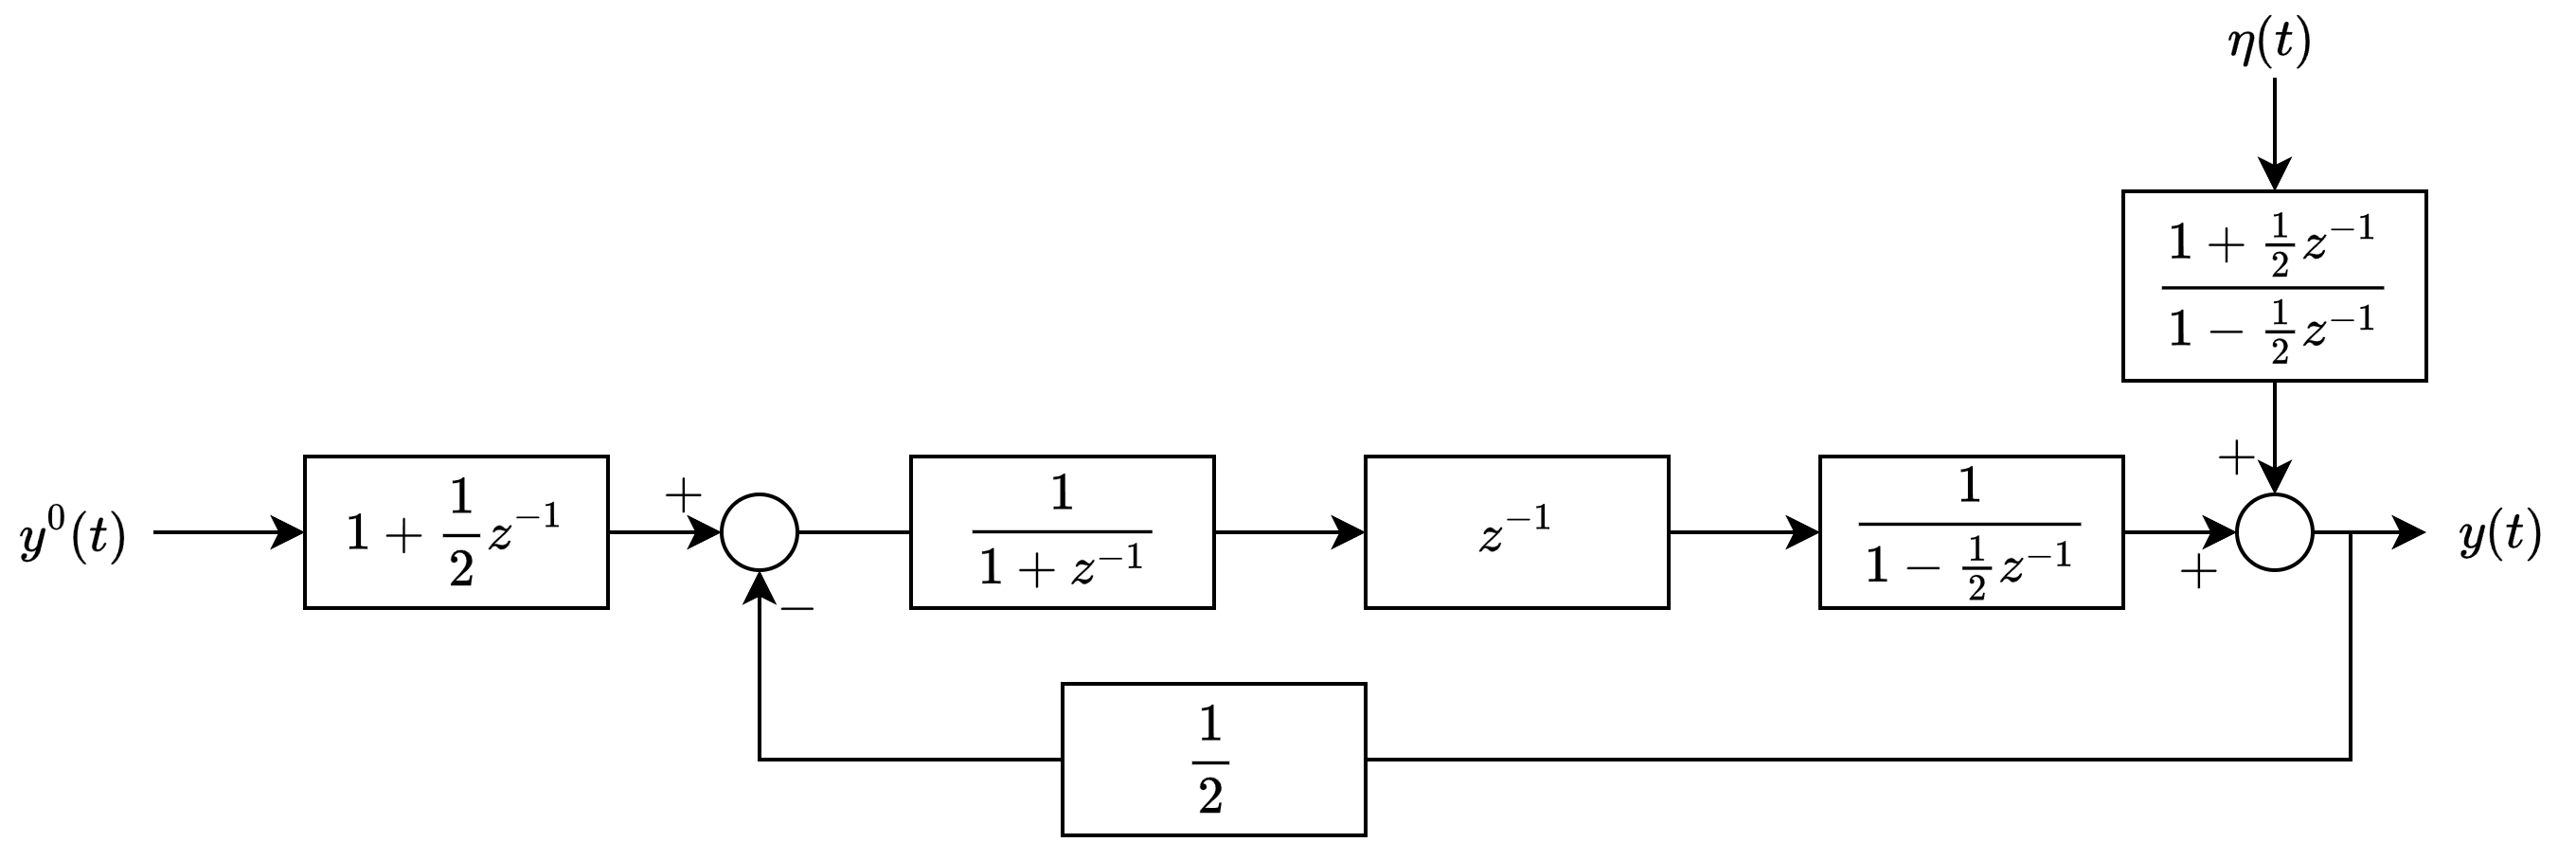
\includegraphics[width=0.75\linewidth]{images/ex3.png}
        \end{figure}
    \item Given the loop transfer function:
        \[L(z)=\dfrac{\frac{1}{2}z^{-2}}{\left(1+z^{-2}\right)\left(1-\frac{1}{2}z^{-1}\right)}\]
        From this, we obtain:
        \[\chi(z)=L_D(z)+L_N(z)=1+\dfrac{1}{2}z^{-1}\]
        Since the root is inside the unit circle, the system is stable.
    \item We calculate the transfer function $W_{y^0u}$ as:
        \[W_{y^0u}=\dfrac{\text{direct path from } y^0(t) \text{ to } u(t)}{1+\text{loop function}}\]
        From the block diagram, we find:
        \[W_{y^0u}=\dfrac{\frac{C(z)}{B(z)E(z)}}{1+\frac{1}{B(z)E(z)}z^{-2}\frac{B(z)}{A(z)}\tilde{R}(z)}=\dfrac{A(z)}{B(z)}\]
    \item From the block diagram, we determine:
        \[W_{\eta u}=\dfrac{-\frac{C(z)\tilde{R}(z)}{B(z)E(z)A(z)}}{\frac{C(z)}{E(z)A(z)}}=-\dfrac{\tilde{R}(z)}{B(z)}\]
        In general, we express the control input $u(t)$ as:
        \[u(t)=-\dfrac{\tilde{R}(z)}{B(z)}\eta(t)+\dfrac{A(z)}{B(z)}y^0(t)\]
\end{enumerate}